\begin{figure}
	\centering
	\setlength{\imagewidth}{0.49\textwidth}%
	\setlength{\imageheight}{0.85\imagewidth}%
	%
	\newdimen\raisevalue
	%
	\DTLsetseparator{,}%
	\DTLloaddb[noheader,keys={x,y}]{dbvertex}{figures/data/pseudo_EdS_sommet/quadpoly/xy_vertex.dat}%
	\DTLloaddb[noheader,keys={x,y}]{dbquadlabel}{figures/data/pseudo_EdS_sommet/quadpoly/xy_quadlabel.dat}%
	\DTLloaddb[noheader,keys={x,y,xl,yl,l}]{dbpointlabel}{figures/data/pseudo_EdS_sommet/quadpoly/xylabel_points.dat}%
	\DTLloaddb[noheader,keys={r,g,b}]{dbcolors}{figures/data/pseudo_EdS_sommet/quadpoly/colors.dat}%
	%
	\pgfmathtruncatemacro\nfaces{\DTLrowcount{dbquadlabel}}
	%
	\pgfmathtruncatemacro\icolor{\nfaces*3}%
	\DTLassign{dbcolors}{\icolor}{\qcolorr=r, \qcolorg=g, \qcolorb=b}%
	\definecolor{quadcolor}{rgb}{\qcolorr, \qcolorg, \qcolorb}
	\colorlet{quadcolordark}{quadcolor!52!black}
	%
	\begin{tikzpicture}[
		x=\imagewidth,
		y=\imageheight,
		img/.style={anchor=south west, inner sep=0},
		curv/.style={line width=0.8pt, line cap=round},
		vector/.style = {-latex', thick},
		label/.style = {font=\small},
		labelpoint/.style = {font=\normalsize},
		insert node/.style args={#1 at #2 raised #3}{
    		postaction=decorate,
    		decoration={
      			markings,
      			mark = at position #2 with {#1},
      			raise = #3
      		}
		}
	]
	%
	\DTLassign{dbvertex}{1}{\vx=x, \vy=y}%
	%
	\begin{scope}
		%
		\node[img] at (0,0) {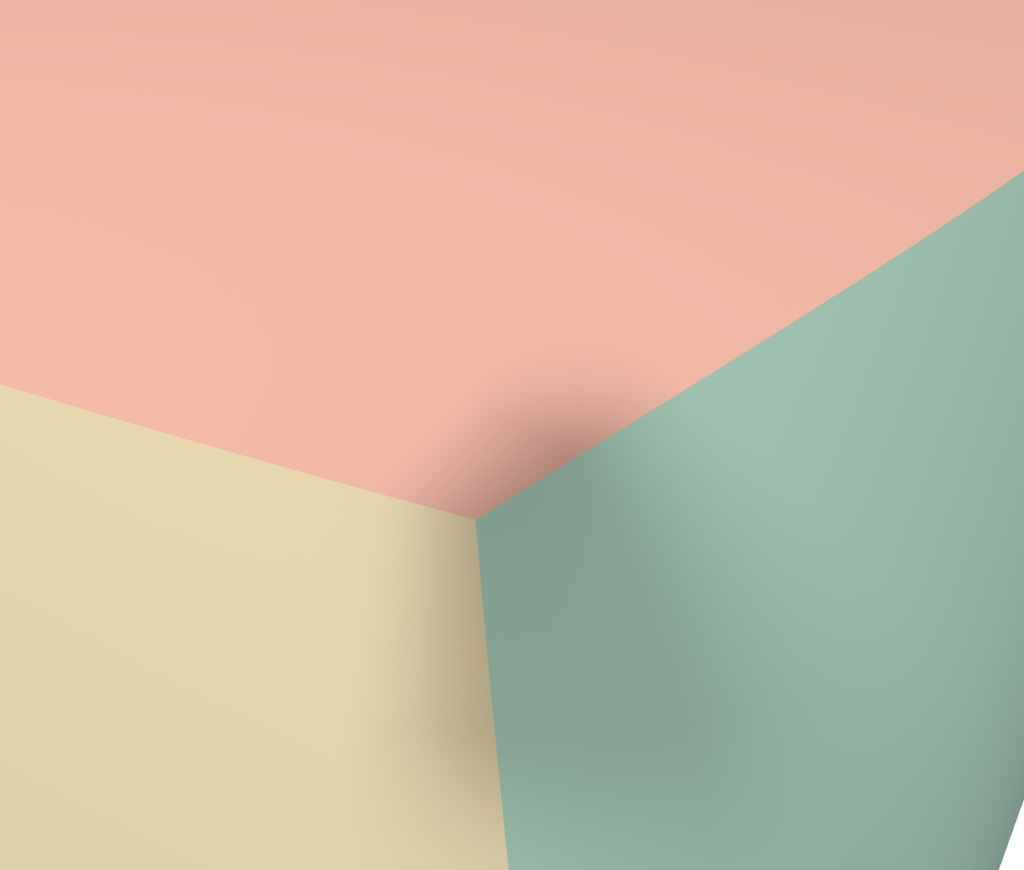
\includegraphics[width=\imagewidth]{pseudo_EdS_sommet/base_shadow}};
		%
		\foreach \iface in {1,...,\nfaces}
		{%
			\DTLassign{dbpointlabel}{\iface}{\px=x, \py=y, \pl=l}%
			\coordinate (p\iface) at ($(\px,\py)$);
			\pgfmathtruncatemacro\iq{\nfaces+\iface}
			\DTLassign{dbpointlabel}{\iq}{\qx=x, \qy=y, \ql=l}%
			\coordinate (q\iface) at ($(\qx,\qy)$);
		}%
		%
		\DTLassign{dbpointlabel}{\DTLrowcount{dbpointlabel}}{\clx=x, \cly=y, \clxl=xl, \clyl=yl, \cll=l}%
		\coordinate (c) at (\clx, \cly);
		{\transparent{0.72}%
			\node[img] at (0,0) {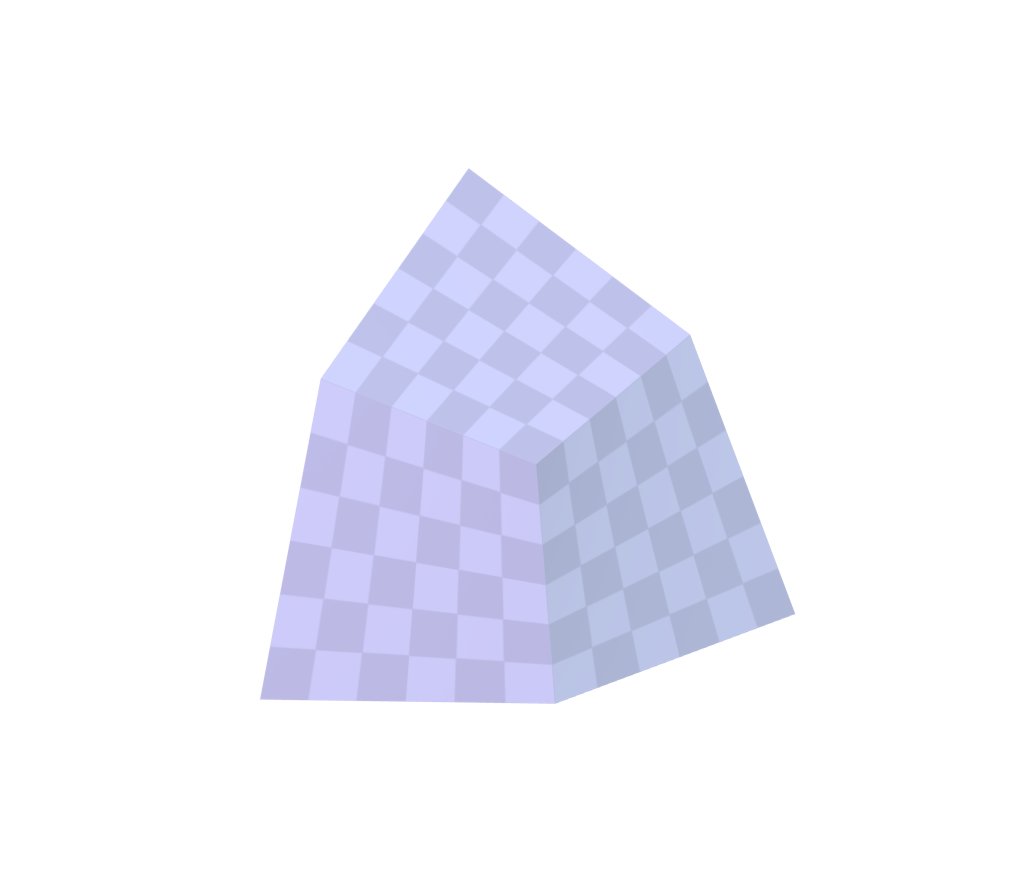
\includegraphics[width=\imagewidth]{pseudo_EdS_sommet/bilinear_only}};
		}%
		%
		\foreach \iface in {1,...,\nfaces}
		{%
			{\transparent{0.8}%
				\draw[
					curv,
					dash pattern=on 2pt off 3pt,
				] plot file {figures/data/pseudo_EdS_sommet/quadpoly/xy_edge_hid_\iface.dat};
			}%
			\draw[
				curv,
				shorten >= 0.4pt,
				insert node={\node[label] {$\brepedge_{\iface}$};} at 0.75 raised -1.8ex,
			] plot file {figures/data/pseudo_EdS_sommet/quadpoly/xy_edge_vis_\iface.dat};
			%
			\DTLassign{dbcolors}{\iface}{\fcolorr=r, \fcolorg=g, \fcolorb=b}%
			\definecolor{facecolor}{rgb}{\fcolorr, \fcolorg, \fcolorb}
			\ifnum \iface=1\relax%
				\colorlet{labelcolor}{facecolor!50!black}
				\raisevalue=1.7ex
			\else%
				\colorlet{labelcolor}{facecolor!60!black}
				\raisevalue=-1.7ex
			\fi%
			%
			\coordinate (n\iface) at ($(\vx, \vy)!0.5!(p\iface)$);
			\draw[vector, labelcolor] (\vx, \vy) -- (n\iface);
			\draw[thick, dotted, labelcolor, shorten <= 1pt] (n\iface) -- (p\iface);
			\path[
				insert node={\node[labelcolor, labelpoint] {$\unv_{\iface}$};} at 0.49 raised -1.7ex,%\raisevalue,
			] (\vx, \vy) -- (p\iface);
			%
			\pgfmathtruncatemacro\jface{1 + mod(\iface, \nfaces)}%
			\draw[thin, quadcolordark]
				(p\iface) -- (q\iface)
				(q\iface) -- (p\jface)
				      (c) -- (q\iface);
		}%
		%
		\DTLforeach{dbpointlabel}{\plx=x, \ply=y, \plxl=xl, \plyl=yl, \pll=l}%
		{%
			\fill[quadcolordark] (\plx, \ply) circle (1.2pt);
			\node[quadcolordark, labelpoint] at (\plxl, \plyl) {$\pll$};
		}%
		%
		%\drawGrid{10}{10}{thin, dotted};
		{\transparent{0.55}%
			\node[label] at (0.90, 0.45) {$\brepface_1$};
			\node[label] at (0.17, 0.85) {$\brepface_2$};
			\node[label] at (0.10, 0.30) {$\brepface_3$};
		}%
		%
		\fill[black] (\vx, \vy) circle (1.2pt);
		\node[above left, labelpoint] at (\vx, \vy) {$\v$};
		%
	\end{scope}
	%
	\begin{scope}[
		shift={(\textwidth-\imagewidth,0)}
	]
		%
		\node[img] at (0,0) {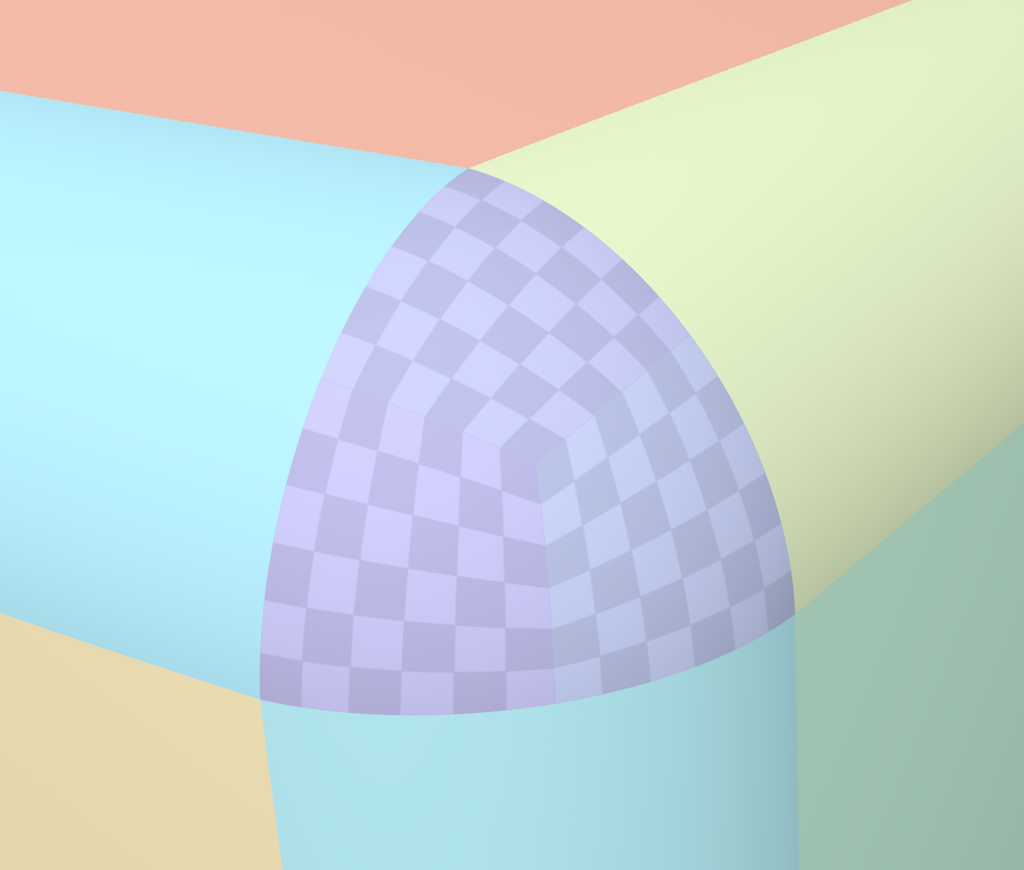
\includegraphics[width=\imagewidth]{pseudo_EdS_sommet/quadpoly}};
		%
		\DTLforeach{dbquadlabel}{\qlx=x, \qly=y}%
		{%
			\pgfmathtruncatemacro\iface{\arabic{DTLrowi}}%
			\pgfmathtruncatemacro\kface{1 + mod(\iface +  \nfaces - 2, \nfaces)}%
			\draw[
				curv,
				insert node={\node[label] {$\Gamma_{\kface,\iface}$};} at 0.25 raised -2ex,
				insert node={\node[label] {$\Gamma_{\iface,\iface}$};} at 0.75 raised -2ex,
			] plot file {figures/data/pseudo_EdS_sommet/quadpoly/xy_arc_\iface.dat};
			\draw[
				curv, 
				shorten >= 0.4pt,
				insert node={\node[label] {$\Gamma_{\iface}$};} at 0.5 raised -1.5ex,
			] plot file {figures/data/pseudo_EdS_sommet/quadpoly/xy_quadsep_\iface.dat};
			%
			{\transparent{0.55}%
				\node[label] at (\qlx, \qly) {$\Sigma_{\iface}$};
			}%
		}%
		%
%		\DTLforeach{dbpointlabel}{\plx=x, \ply=y, \plxl=xl, \plyl=yl, \pll=l}%
%		{%
%			\fill[black] (\plx, \ply) circle (1.2pt);
%			\node[labelpoint] at (\plxl, \plyl) {$\pll$};
%		}%
		%
		%\drawGrid{10}{10}{thin, dotted};
		{\transparent{0.55}%
			\node[label] at (0.90, 0.20) {$\EdSpropreplus{\brepface_1}{\rho}$};
			\node[label] at (0.45, 0.92) {$\EdSpropreplus{\brepface_2}{\rho}$};
			\node[label] at (0.10, 0.10) {$\EdSpropreplus{\brepface_3}{\rho}$};
			%
			\node[label] at (0.55, 0.05) {$\pseudoEdS{\brepedge_1}{\rho}$};
			\node[label] at (0.85, 0.74) {$\pseudoEdS{\brepedge_2}{\rho}$};
			\node[label] at (0.13, 0.58) {$\pseudoEdS{\brepedge_3}{\rho}$};
		}%
	\end{scope}
	%
	\end{tikzpicture}
	\DTLgdeletedb{dbvertex}%
	\DTLgdeletedb{dbquadlabel}%
	\DTLgdeletedb{dbpointlabel}%
	\DTLgdeletedb{dbcolors}%
	%
	\caption{Représentation de la pseudo-EdS d'un sommet à l'aide de plusieurs carreaux non-restreints.}
	\label{fig:pseudo_EdS_sommet_quadpoly}
\end{figure}